\documentclass[a4paper,12pt]{article}
\usepackage[utf8]{inputenc}
\usepackage[brazil]{babel}
\usepackage{graphicx}
\usepackage[top=0.5cm,bottom=2.5cm,left=2.5cm,right=2.5cm]{geometry}

\newcommand{\assinatura}[2]{%
\begin{center}
\hrulefill\\
\textbf{#2: #1}
\par \hfill
\par \hfill
\end{center}
}

\newcommand{\nomeorientador}{} % storage macro
\newcommand{\orientador}[1]{%
  \renewcommand{\nomeorientador}{#1}%
}

\newcommand{\nomealuno}{} % storage macro
\newcommand{\aluno}[1]{%
  \renewcommand{\nomealuno}{#1}%
}

\newcommand{\matricula}{} % storage macro
\newcommand{\numeromatricula}[1]{%
  \renewcommand{\matricula}{#1}%
}

\newcommand{\nomebancaum}{} % storage macro
\newcommand{\bancaum}[1]{%
  \renewcommand{\nomebancaum}{#1}%
}

\newcommand{\nomebancadois}{} % storage macro
\newcommand{\bancadois}[1]{%
  \renewcommand{\nomebancadois}{#1}%
}

\newcommand{\nomebancatres}{} % storage macro
\newcommand{\bancatres}[1]{%
  \renewcommand{\nomebancatres}{#1}%
}

\newcommand{\notatcc}{} % storage macro
\newcommand{\notaavaliada}[1]{%
  \renewcommand{\notatcc}{#1}%
}

\newcommand{\titulotcca}{} % storage macro
\newcommand{\nometcca}[1]{%
  \renewcommand{\titulotcca}{#1}%
}
\newcommand{\titulotccb}{} % storage macro
\newcommand{\nometccb}[1]{%
  \renewcommand{\titulotccb}{#1}%
}
\newcommand{\titulotccc}{} % storage macro
\newcommand{\nometccc}[1]{%
  \renewcommand{\titulotccc}{#1}%
}
\newcommand{\localdefesa}{} % storage macro
\newcommand{\saladefesa}[1]{%
  \renewcommand{\localdefesa}{#1}%
}

\orientador{Janio Rosa da Silva}
\aluno{Guilherme Henrique Costa Vieira}
\numeromatricula{0100789}
\bancaum{Adilson Ribeiro de Oliveira}
\bancadois{Joaquim Eduardo de Moura}
%\bancatres{Márcio Assis Miranda}
\notaavaliada{100,00}
%\nometcc1{Tradição e Memória Cultural na Toponimia Urbana de Ouro Branco: A Transposição Computacional do Acervo Cultural do Município}
\nometcca{Dispositivo discreto de acionamento de emergência}
\nometccb{ para mulheres em situação de violência doméstica}
\nometccc{}
\saladefesa{do Google Meetings}
\begin{document}

% ===== HEADER PAGE 1 =====
%\begin{center}
%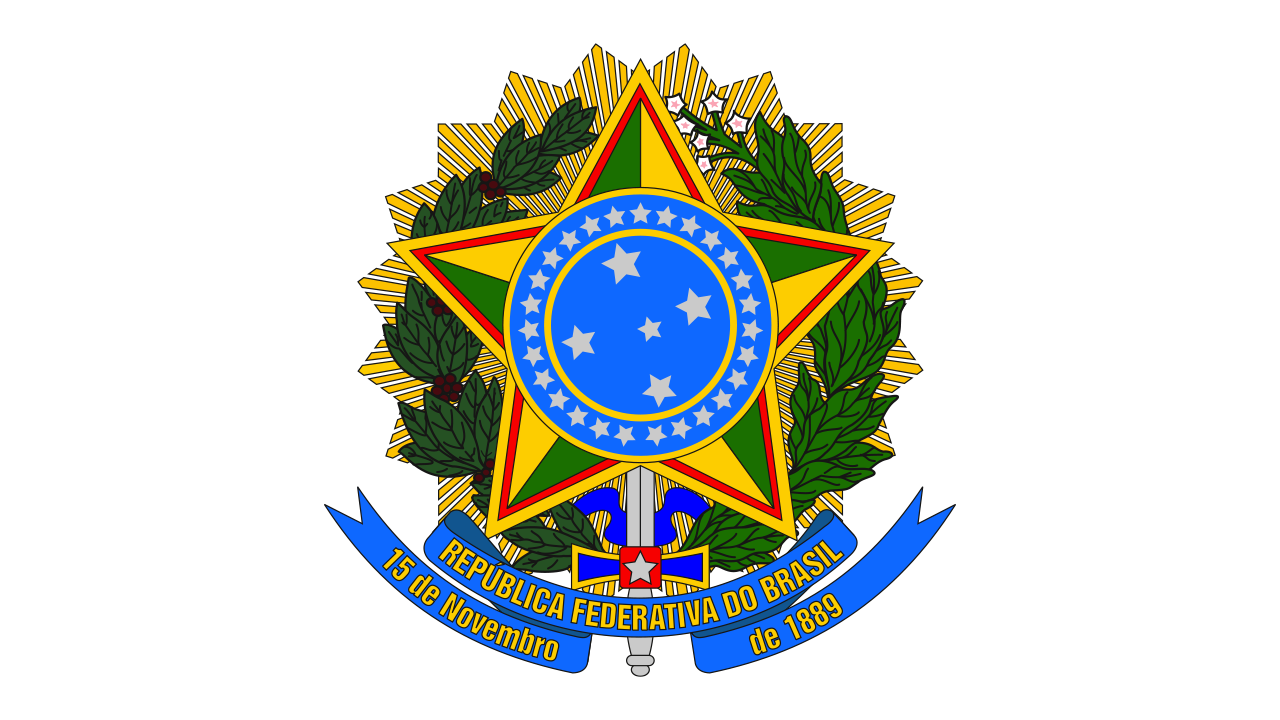
\includegraphics[width=0.4\textwidth]{image.png}
%
%\textbf{MINISTÉRIO DA EDUCAÇÃO}\\
%\textbf{SECRETARIA DE EDUCAÇÃO PROFISSIONAL E TECNOLÓGICA}\\
%\textbf{INSTITUTO FEDERAL DE EDUCAÇÃO, CIÊNCIA E TECNOLOGIA DE MINAS %GERAIS}\\
%\textbf{CAMPUS OURO BRANCO}\\
%Av. Afonso Sardinha, nº 90, Bairro Pioneiros, CEP: 36.420-000, Ouro %Branco - Minas Gerais\\
%(31) 3742-2149 – gabinete.ourobranco@ifmg.edu.br
%\end{center}

%\vspace{0.8cm}

%\begin{center}
%\textbf{ANEXO II – ATA DE CONCLUSÃO DE TCC}
%\end{center}

%Aos \underline{\textbf{10}} dias do mês de \underline{\textbf{Julho}} de %\underline{\textbf{2026}}, às \underline{\textbf{15:00}} horas,  
%\underline{\textbf{\nomealuno}}, aluno(a) regularmente matriculado no %Curso de Sistemas de Informação do Instituto Federal de Minas Gerais, %campus Ouro Branco, matrícula \underline{\textbf{\matricula}}, concluiu %o seu Trabalho de Conclusão de Curso por meio de:

%\vspace{0.4cm}

%\fbox{
%\begin{minipage}{0.96\textwidth}

%( ) Publicação do artigo intitulado \hrulefill  
%na revista/conferência \hrulefill,  
%cujo comprovante de aceitação será anexado a esta ata, recebendo a nota %\hrulefill pelo trabalho. Eu, na qualidade de orientador do aluno, lavrei %a presente ata atestando a conclusão do trabalho, a qual será assinada %por mim e pelo aluno.

%\vspace{0.5cm}

%Professor Orientador: \hrulefill  

%Aluno: \hrulefill  

%\vspace{0.5cm}

%(\underline{\textbf{X}}) Defesa em sessão pública realizada às %%\underline{\textbf{15:00}} horas, na sala %\underline{\textbf{\localdefesa}} do Instituto Federal de Minas Gerais, %campus Ouro Branco, na presença da banca examinadora composta pelos %docentes:

%\underline{\textbf{1 - \nomebancaum}}\\
%\underline{\textbf{2 - \nomebancadois}}\\
%\underline{\textbf{3 - \nomeorientador}}\\
%\underline{\textbf{3 - \nomebancatres}}\\

%do artigo intitulado \underline{\textbf{\titulotcca}}\\  
%\underline{\textbf{\titulotccb}}\\
%\underline{\textbf{\titulotccc}}\\
%\underline{\textbf{do ENEM Baseado em Teoria de Resposta ao Item}}\\  
%\end{minipage}
%}

%\newpage

% ===== HEADER PAGE 2 =====
%\begin{center}
%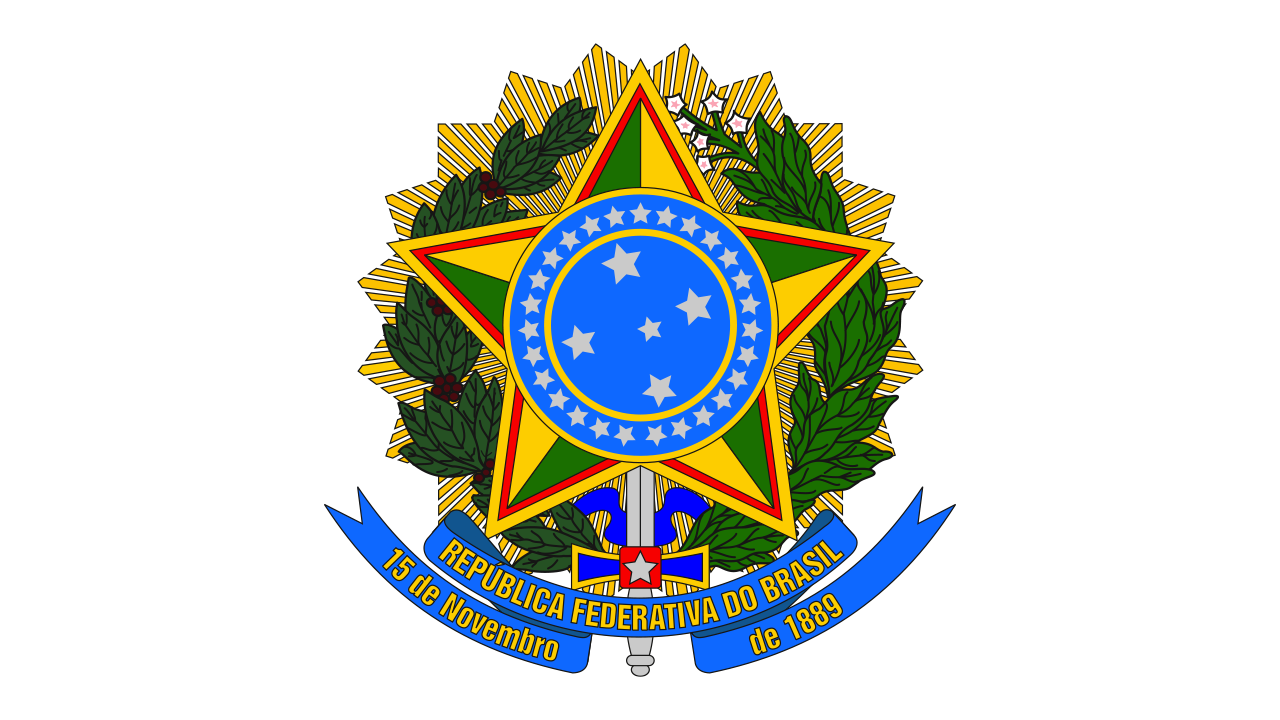
\includegraphics[width=0.4\textwidth]{image.png}

%\textbf{MINISTÉRIO DA EDUCAÇÃO}\\
%\textbf{SECRETARIA DE EDUCAÇÃO PROFISSIONAL E TECNOLÓGICA}\\
%\textbf{INSTITUTO FEDERAL DE EDUCAÇÃO, CIÊNCIA E TECNOLOGIA DE MINAS %GERAIS}\\
%\textbf{CAMPUS OURO BRANCO}\\
%Av. Afonso Sardinha, nº 90, Bairro Pioneiros, CEP: 36.420-000, Ouro %Branco - Minas Gerais\\
%(31) 3742-2149 – gabinete.ourobranco@ifmg.edu.br
%\end{center}

%\vspace{0.8cm}

%\fbox{
%\begin{minipage}{0.96\textwidth}

%A banca examinadora, após reunião em sessão reservada, deliberou pela %\underline{\textbf{Aprovação}} do referido trabalho, atribuindo a nota \underline{\textbf{\notatcc}}. Eu, na qualidade de presidente da banca %examinadora, lavrei a presente ata que será assinada por mim, pelos %demais examinadores e pelo aluno.

%\vspace{0.5cm}

%Observações pertinentes à defesa:  
%\hrulefill  
%\hrulefill  

%\vspace{0.5cm}

%\begin{center}
%\textbf{NOME E ASSINATURA DOS COMPONENTES DA BANCA E DO ORIENTADO}
%\end{center}

%\vspace{0.3cm}

%\assinatura{\nomeorientador}{Orientador}
%\assinatura{\nomebancaum}{Examinador 1}
%\assinatura{\nomebancadois}{Examinador 2}
%\assinatura{\nomebancatres}{Examinador 3}
%\assinatura{\nomealuno}{Aluno}


%\end{minipage}
%}
% ===== HEADER PAGE 3 =====
\begin{center}
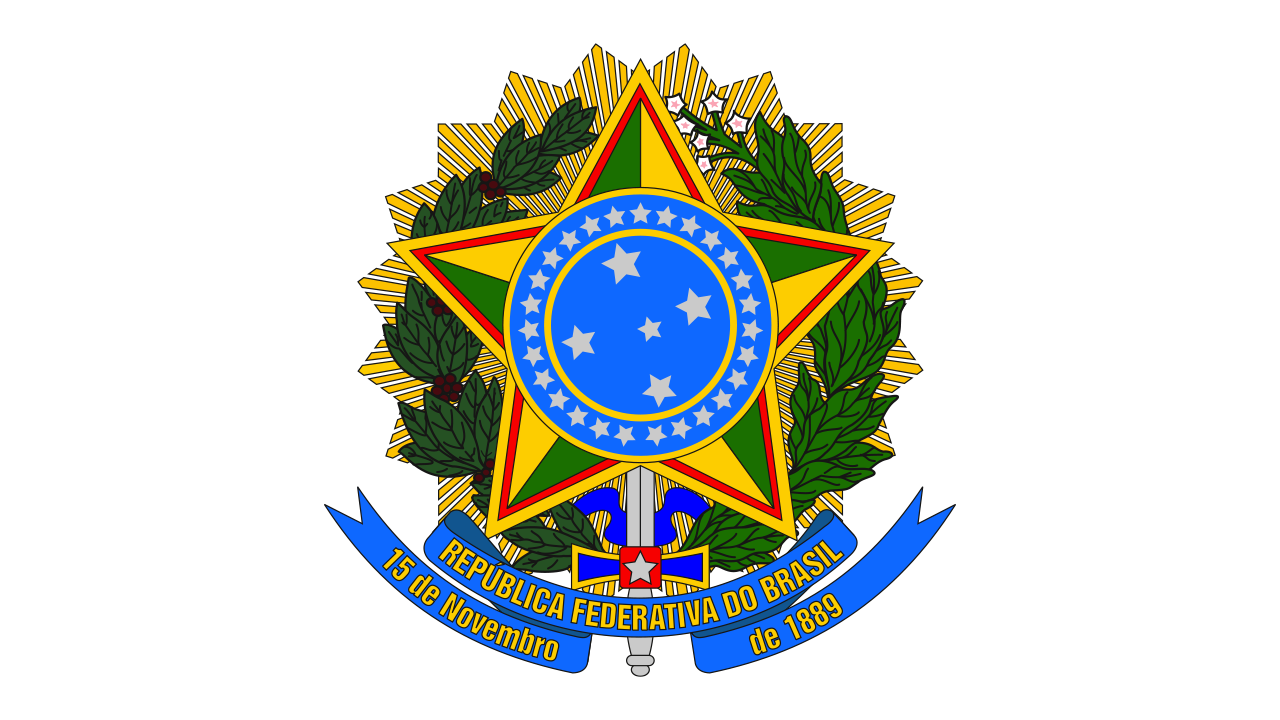
\includegraphics[width=0.4\textwidth]{image.png}

\textbf{MINISTÉRIO DA EDUCAÇÃO}\\
\textbf{SECRETARIA DE EDUCAÇÃO PROFISSIONAL E TECNOLÓGICA}\\
\textbf{INSTITUTO FEDERAL DE EDUCAÇÃO, CIÊNCIA E TECNOLOGIA DE MINAS GERAIS}\\
\textbf{CAMPUS OURO BRANCO}\\
Av. Afonso Sardinha, nº 90, Bairro Pioneiros, CEP: 36.420-000, Ouro Branco - Minas Gerais - (31) 3742-2149 – gabinete.ourobranco@ifmg.edu.br
\end{center}

\vspace{0.8cm}

\textbf{DECLARAÇÃO ANTI-PLÁGIO}

\vspace{0.3cm}

Eu, \underline{\textbf{\nomealuno}}, matrícula \underline{\textbf{\matricula}}, estudante do curso Bacharelado em Sistemas de Informação do IFMG – Campus Ouro Branco, declaro, para os devidos fins e efeitos, e para fazer prova junto ao IFMG – Campus Ouro Branco, que, \textbf{sob as penalidades previstas no art. 299 do Código Penal Brasileiro}, que é de minha criação o Trabalho de Conclusão de Curso que ora apresento.

\textbf{Art. 299 do Código Penal Brasileiro, que dispõe sobre o crime de Falsidade Ideológica:}

“Omitir, em documento público ou particular, declaração que dele devia constar, ou nele inserir ou fazer inserir declaração falsa ou diversa da que devia estar escrita, com o fim de prejudicar direito, criar obrigação ou alterar verdade sobre fato juridicamente relevante:

Pena – reclusão, de 1 (um) a 5 (cinco) anos, e multa, se o documento é público, e reclusão de 1 (um) a 3 (três) anos, e multa, se o documento é particular.

Parágrafo único. Se o agente é funcionário público, e comete o crime prevalecendo-se do cargo, ou se a falsificação ou alteração é de assentamento de registro civil, aumenta-se a pena de sexta parte”.

Este crime engloba plágio e compra fraudulenta de documentos científicos. Por ser verdade, e por ter ciência do referido artigo, firmo a presente declaração.

\vspace{0.8cm}

Ouro Branco, \underline{\textbf{14}} de \underline{\textbf{Julho}} de \underline{\textbf{2026}}  

\vspace{0.5cm}
\par \hfill \\
\textbf{Assinatura do aluno:} \hrulefill

\end{document}
